% conclusion / synthèse


\begin{frame}{Inférer des réseaux de régulation : un tâche encore complexe}
	
	\begin{enumerate}
	    \item Problème en grande dimension
	    
	    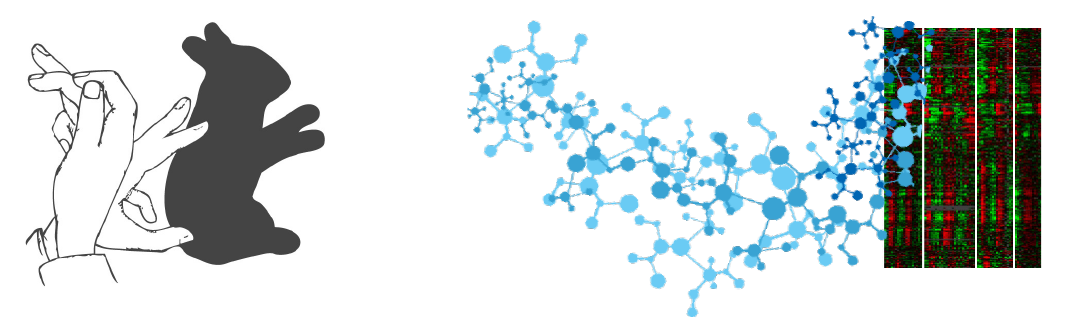
\includegraphics[scale=0.2]{Figures/Intro/shadowplay.png}
	    
	    
	    \item Manque de données de validation complètes et sûres pour étalonner les méthodes
	\end{enumerate}

\end{frame}




\begin{frame}{Combiner plusieurs approches d'inférence}

\scriptsize En 2012, les challenges \textbf{DREAM} ont évalué et combiné l'état de l'art des méthodes d'inférence  et conclu à un apport significatif de la combinaison de plusieurs méthodes [Marbach et al., 2012]

\centering
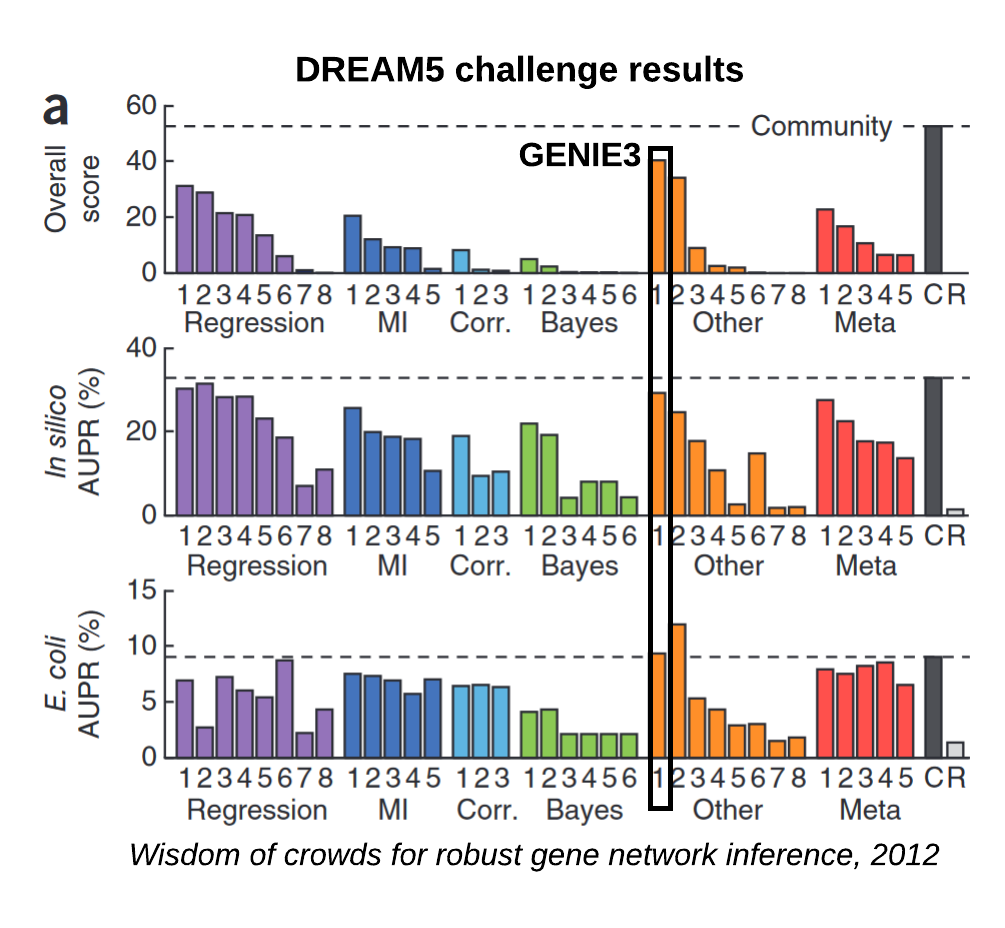
\includegraphics[scale = 0.38]{Figures/Regression/dream5.png}
\end{frame}






% DREAM

% Utilisation d'informations a priori

% adaptation temporelle

% ouverture sur DIANE